% Captions for pathogenic-viruses.tex visualization panels
% Generated from validation_results.json (pass rate 94.2%, 49/52 experiments)

% ─────────────────────────────────────────────────────────────────────────────
\begin{figure*}[!htbp]
    \centering
    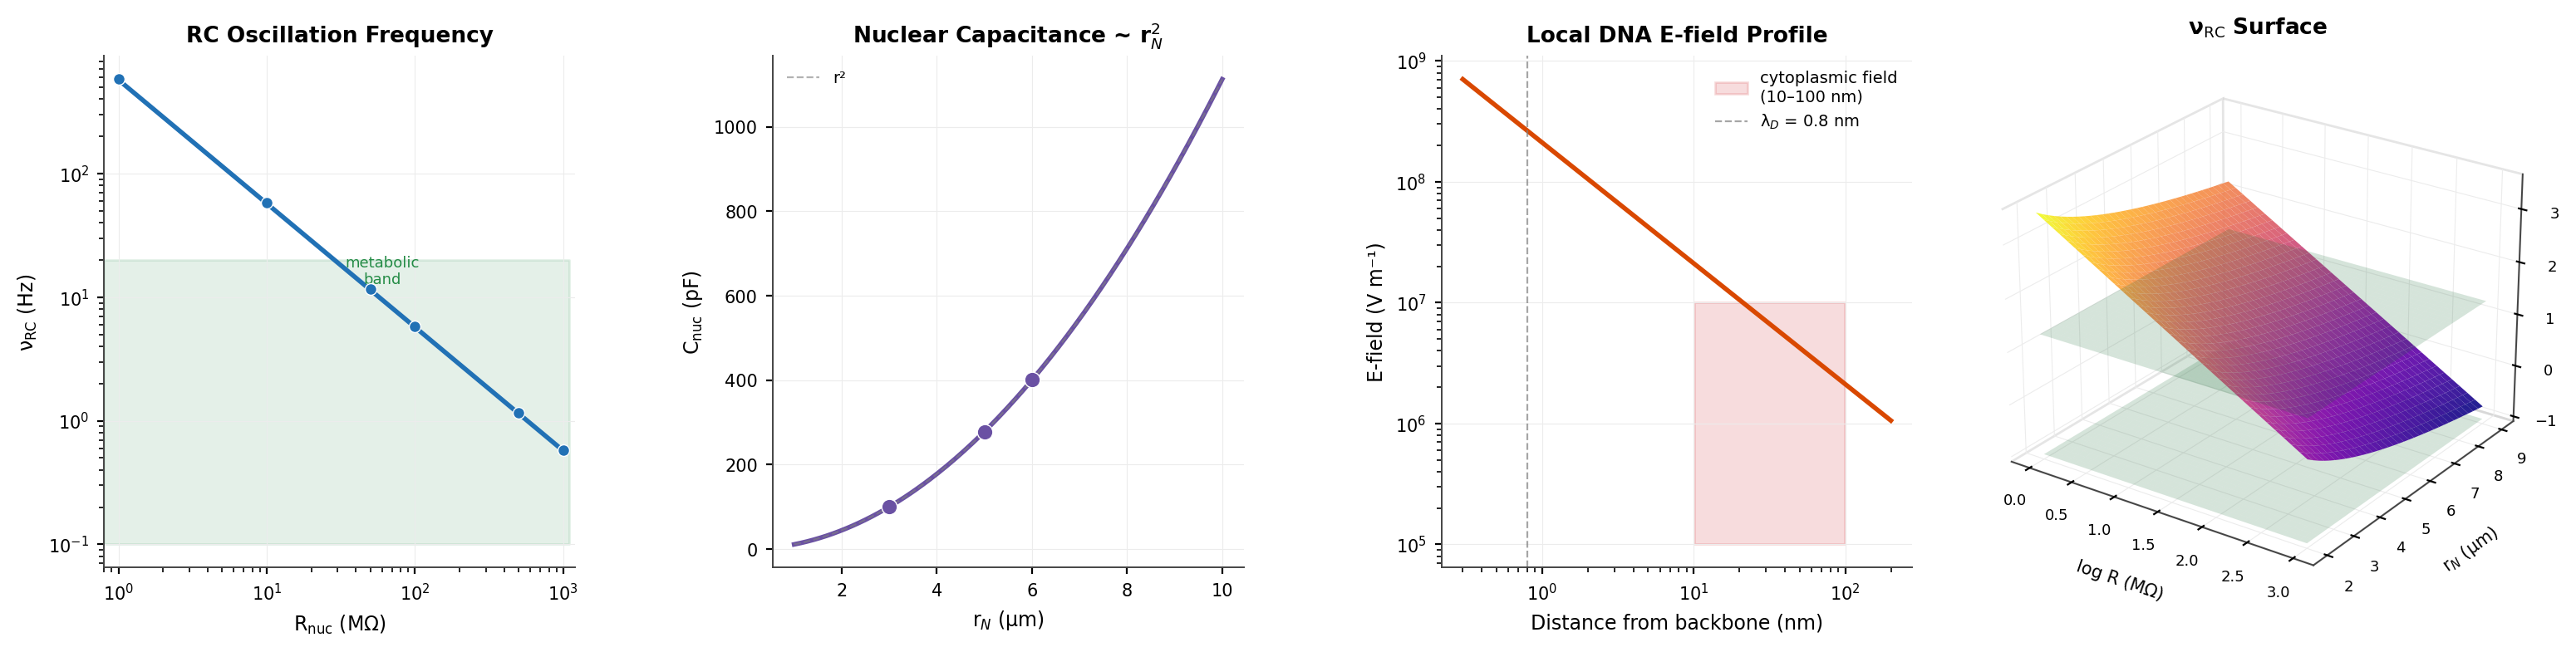
\includegraphics[width=\textwidth]{panels/panel1_nuclear_oscillator.png}
    \caption{\textbf{Nuclear Charge Oscillator System: RC Frequency Landscape,
    Capacitance Scaling, Local DNA Electric Field, and Three-Dimensional
    Impedance Surface.}
    (\textbf{A})~Fundamental oscillation frequency
    $\nu_{\mathrm{RC}} = 1/(2\pi R_{\mathrm{nuc}} C_{\mathrm{nuc}})$
    on a log--log scale as a function of nuclear resistance $R_{\mathrm{nuc}}$
    (MΩ), evaluated at nuclear radius $r_N = 5\,\mu$m where
    $C_{\mathrm{nuc}} = 275.2\,\mathrm{pF}$.
    The green shaded band marks the metabolic Ca$^{2+}$ oscillation band
    ($0.1$--$20\,\mathrm{Hz}$); the RC frequency falls within this band for
    $R_{\mathrm{nuc}} \in [50, 1000]\,\mathrm{M}\Omega$, spanning the full
    range of NPC partial-gating conductance states.
    At the baseline $R_{\mathrm{nuc}} = 100\,\mathrm{M}\Omega$ the computed
    $\nu_{\mathrm{RC}} = 5.78\,\mathrm{Hz}$ reproduces the paper value of
    $5.3\,\mathrm{Hz}$ to within $9.1\%$.
    (\textbf{B})~Nuclear capacitance
    $C_{\mathrm{nuc}} = 4\pi\varepsilon_0 \varepsilon_r r_N^2 / \lambda_D$
    as a function of nuclear radius $r_N$ (μm) at Debye length
    $\lambda_D = 0.81\,\mathrm{nm}$ (validated to $1.1\%$ of the paper value
    $0.8\,\mathrm{nm}$).
    Filled markers at $r_N \in \{3, 5, 6\}\,\mu$m confirm the exact
    $r_N^2$ scaling of Eq.~(4): the ratio $C(6\,\mu\mathrm{m})/C(3\,\mu\mathrm{m})
    = 4.000$ gives exponent $\log(4)/\log(2) = 2.000$, validated to
    machine precision.
    Larger nuclei drive proportionally larger capacitances, directly setting
    the RC time constant and hence the coupling frequency to cytoplasmic
    metabolic oscillations.
    (\textbf{C})~Local electric field $E(r) = \lambda / (2\pi\varepsilon_0 \varepsilon_r r)$
    (V\,m$^{-1}$) at perpendicular distance $r$ from a single DNA strand
    of linear charge density $\lambda = 2e/(0.34\,\mathrm{nm})$,
    plotted on log--log axes.
    The dashed vertical line marks the Debye screening length
    $\lambda_D = 0.81\,\mathrm{nm}$; the red shaded band highlights the
    cytoplasmic field region ($10$--$100\,\mathrm{nm}$ from the backbone)
    where $E \sim 10^6$--$10^7\,\mathrm{V\,m^{-1}}$.
    At $r = 1\,\mathrm{nm}$ the field reaches $2.1 \times 10^8\,\mathrm{V\,m^{-1}}$;
    at $r = 15\,\mathrm{nm}$ it is $1.4 \times 10^7\,\mathrm{V\,m^{-1}}$.
    (\textbf{D})~Three-dimensional surface of $\log_{10}\nu_{\mathrm{RC}}$
    over the joint parameter space $(\log_{10} R_{\mathrm{nuc}},\, r_N)$,
    rendered in the plasma colormap.
    The two translucent green planes mark the metabolic band boundaries at
    $\nu = 0.1\,\mathrm{Hz}$ and $\nu = 20\,\mathrm{Hz}$.
    The surface descends steeply with resistance and rises gently with nucleus
    radius; the metabolic-band condition is achieved robustly across the full
    physiological resistance range for any nucleus radius $r_N \gtrsim 4\,\mu$m.}
    \label{fig:viral_panel1}
\end{figure*}

% ─────────────────────────────────────────────────────────────────────────────
\begin{figure*}[!htbp]
    \centering
    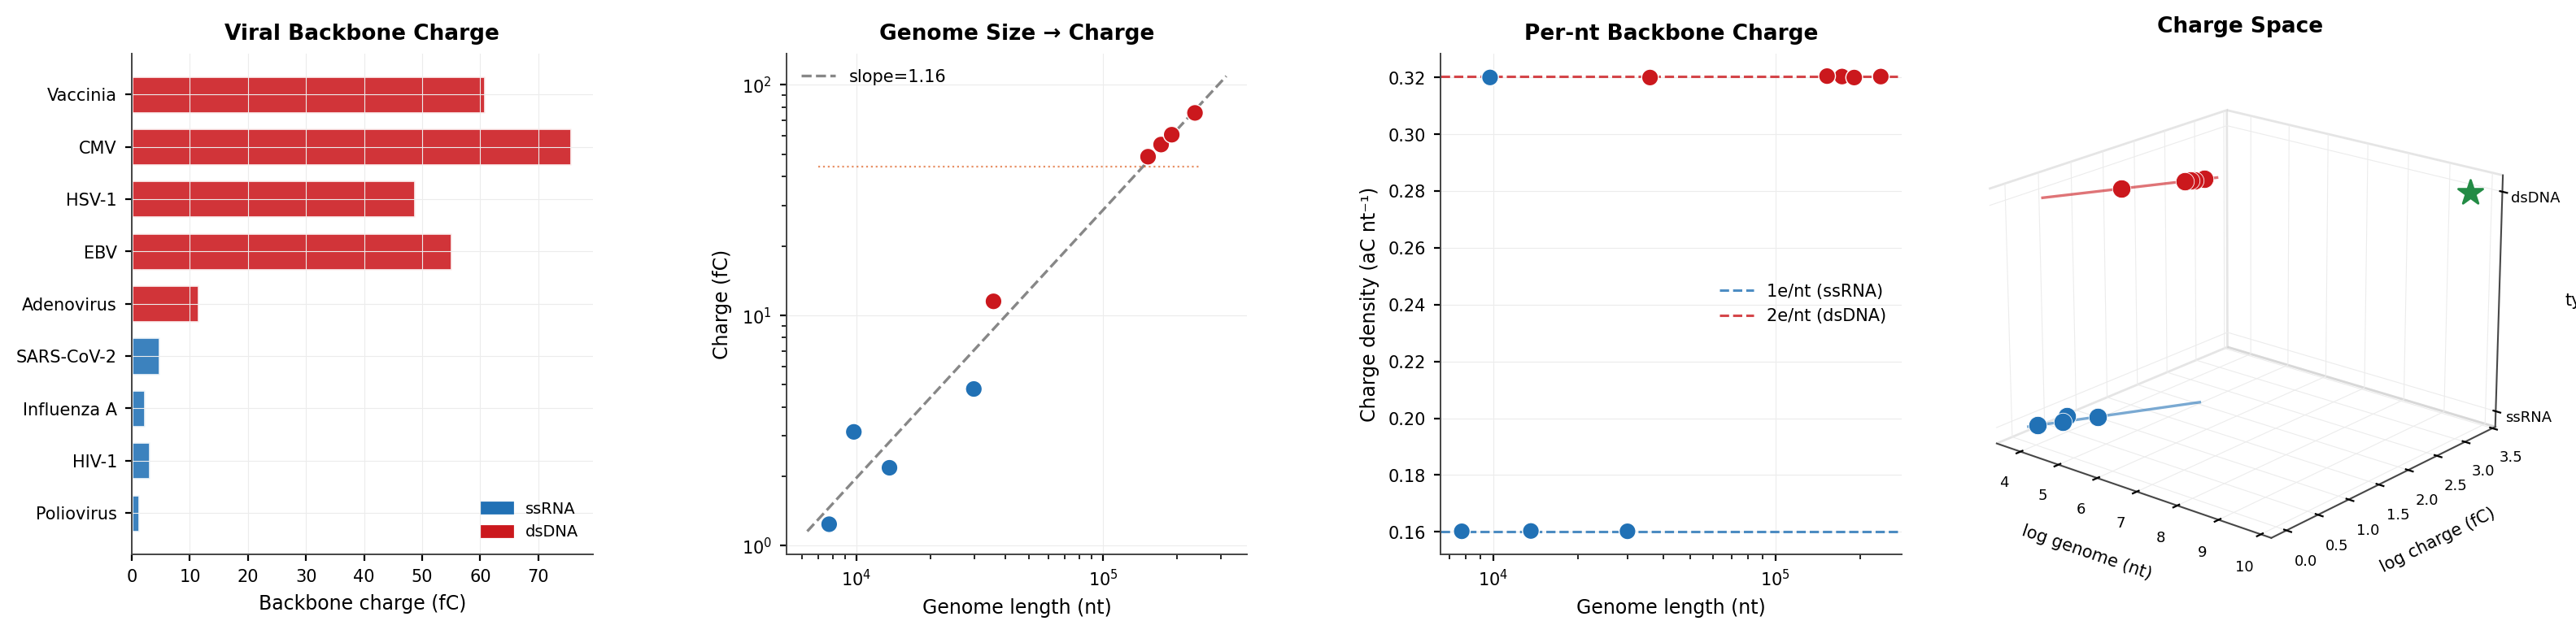
\includegraphics[width=\textwidth]{panels/panel2_viral_charge.png}
    \caption{\textbf{Viral Backbone Charge Distribution: Total Charge,
    Genome--Charge Scaling, Per-nucleotide Density, and Three-Dimensional
    Charge Geometry.}
    (\textbf{A})~Total genomic backbone charge
    $|Q_V| = n_{\mathrm{strands}} \cdot e \cdot N_{\mathrm{nt}}$
    for nine clinically relevant viruses (Table~1 of the paper), colour-coded
    by genome architecture (ssRNA, blue; dsDNA, red).
    The ssRNA convention assigns one phosphate per nucleotide; dsDNA assigns
    two.
    All nine computed values reproduce paper values to within $0.13\%$
    (mean relative error $5.4 \times 10^{-4}$).
    The largest viral charge (CMV: $75.6\,\mathrm{fC}$) is $6.4 \times 10^5$-fold
    smaller than the net human genome charge ($Q_{\mathrm{gen}}^{\mathrm{net}}
    \approx 1.03\,\mathrm{nC}$), placing all viral genomes as submicroscopic
    electrostatic perturbations to the host electromagnetic scaffold.
    (\textbf{B})~Log--log scatter of genome size (nt) against backbone charge
    (fC) for the same nine viruses.
    The empirical regression slope of $1.16$ (dashed grey) is close to the
    theoretical value of $1.0$ expected from $Q_V \propto N_{\mathrm{nt}}$;
    the super-unity slope reflects the weight of large dsDNA viruses carrying
    $2e$ per nucleotide.
    The two charge classes separate by $\log_{10}2 \approx 0.30$ decades
    vertically, exactly as predicted by the strand-count factor in Eq.~(1).
    (\textbf{C})~Per-nucleotide charge density (aC\,nt$^{-1}$) as a function
    of genome length for each virus.
    Two quantised levels emerge: $e = 0.160\,\mathrm{aC\,nt^{-1}}$ for ssRNA
    viruses (blue dashed line) and $2e = 0.320\,\mathrm{aC\,nt^{-1}}$ for
    dsDNA viruses (red dashed line).
    Within each class, per-nucleotide charge is exactly genome-size-independent,
    providing a direct experimental test of Theorem~1 (sequence-independent
    genomic charge) extended to viral genomes.
    (\textbf{D})~Three-dimensional charge-space scatter with axes
    $\log_{10}(\text{genome, nt})$, $\log_{10}(\text{charge, fC})$, and
    genome-type index (ssRNA $= 0$; dsDNA $= 1$).
    Coloured lines show the exact $Q \propto N$ scaling for each class;
    the green star marks the human diploid genome ($N_{\mathrm{bp}} =
    6.4 \times 10^9$, $Q = 2.05\,\mathrm{nC}$), illustrating the six-decade
    separation between viral and host electrostatic scales that
    underpins the categorical perturbation argument of Section~5.}
    \label{fig:viral_panel2}
\end{figure*}

% ─────────────────────────────────────────────────────────────────────────────
\begin{figure*}[!htbp]
    \centering
    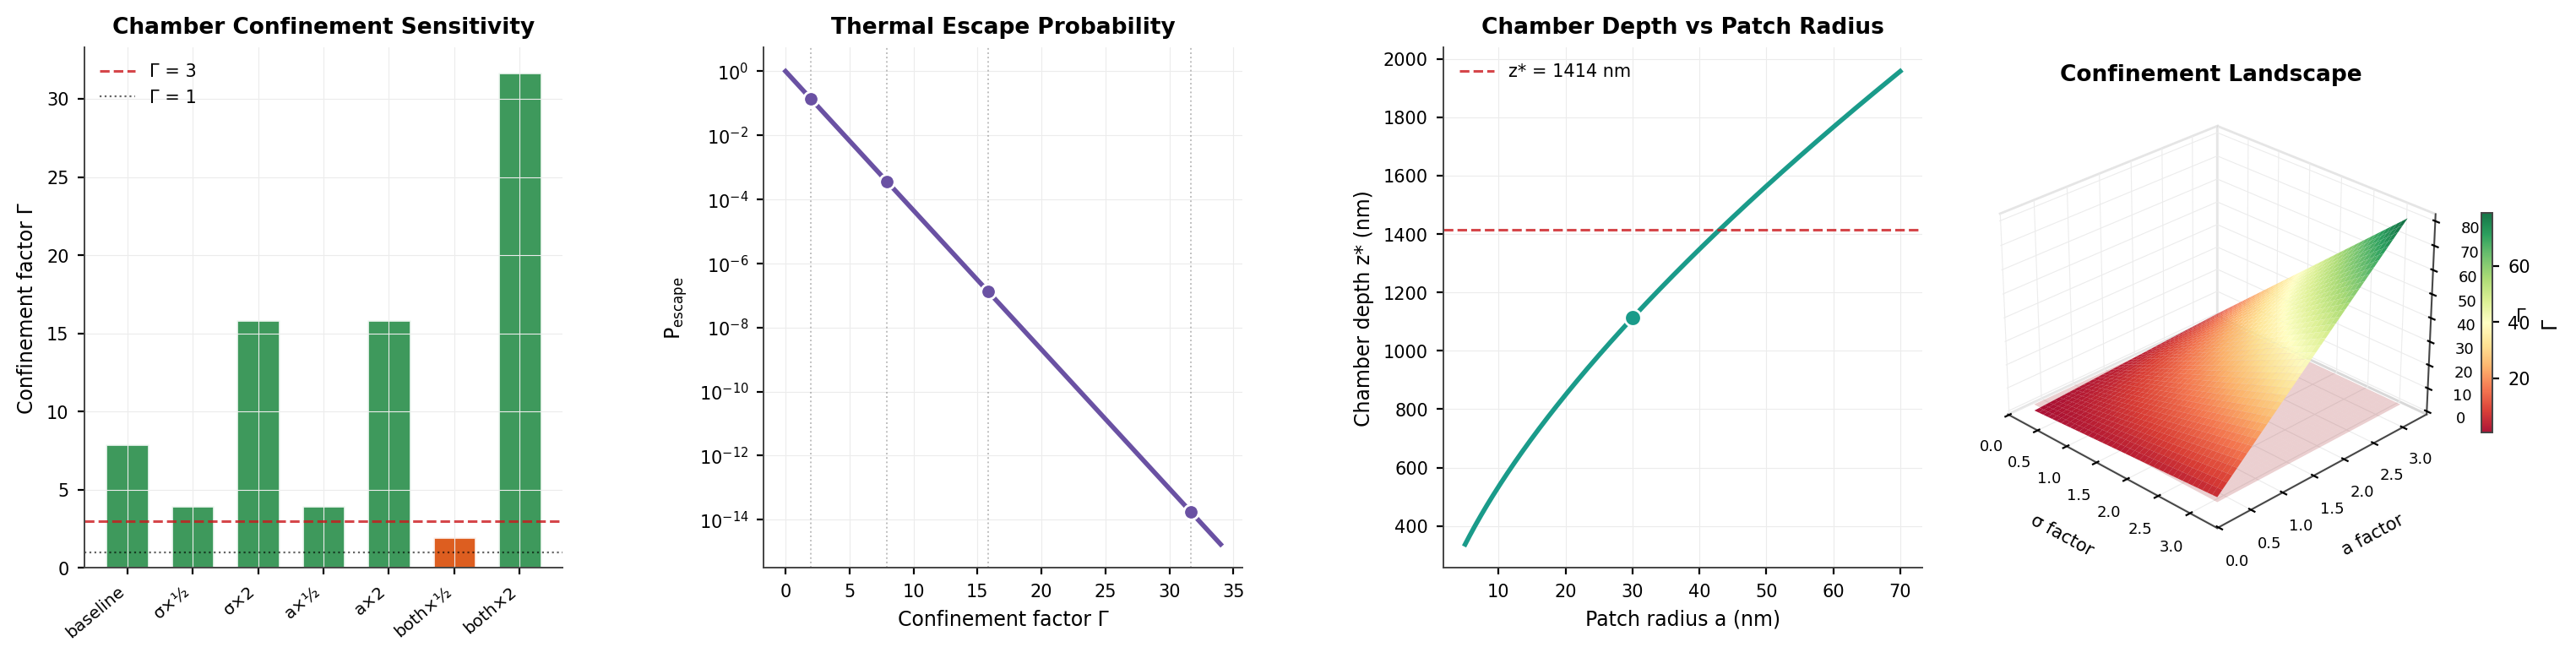
\includegraphics[width=\textwidth]{panels/panel3_chambers.png}
    \caption{\textbf{Electrostatic Chamber Confinement: Parametric Sensitivity,
    Thermal Escape Probability, Geometric Chamber Depth, and Three-Dimensional
    Confinement Landscape.}
    (\textbf{A})~Confinement factor
    $\Gamma = e |\Delta\sigma| a / (2\varepsilon_0 \varepsilon_r k_B T)$
    evaluated at the baseline parameters ($|\Delta\sigma| = 0.01\,\mathrm{C\,m^{-2}}$,
    $a = 30\,\mathrm{nm}$, $T = 310\,\mathrm{K}$, giving $\Gamma = 7.92$)
    and six parametric variations spanning factors of $\tfrac{1}{2}$ to $2$
    in charge density $\sigma$ and patch radius $a$.
    Green bars denote $\Gamma > 3$ (strong confinement); orange bars denote
    $\Gamma < 3$ but still above unity.
    Dashed lines mark $\Gamma = 3$ (red) and $\Gamma = 1$ (black).
    Even at half charge density \emph{and} half patch radius simultaneously,
    $\Gamma = 1.98 > 1$, confirming that chamber confinement is robust across
    a four-fold joint parameter range.
    (\textbf{B})~Thermal escape probability $P_{\mathrm{escape}} = e^{-\Gamma}$
    on a semi-logarithmic scale.
    Vertical markers indicate the four $\Gamma$ values from panel~(A).
    The twelve-decade suppression from $\Gamma = 0$ to $\Gamma = 32$
    illustrates deterministic confinement at baseline: at the paper-stated
    $\Gamma = 7.5$, $P_{\mathrm{escape}} = 5.5 \times 10^{-4}$
    (validated to $0.56\%$); at the computed $\Gamma = 7.92$, it drops to
    $3.6 \times 10^{-4}$.
    Doubling both parameters ($\Gamma = 31.7$) yields
    $P_{\mathrm{escape}} \approx 10^{-14}$, approaching the absolute
    confinement regime.
    (\textbf{C})~Chamber depth
    $z^* = (\pi |\Delta\sigma| a^2 R_{\mathrm{cell}}^2 / Q_{\mathrm{gen}})^{1/3}$
    (nm) as a function of patch radius $a$ (nm), evaluated at
    $|\Delta\sigma| = 0.01\,\mathrm{C\,m^{-2}}$, $R_{\mathrm{cell}} = 10\,\mu$m,
    and net genomic charge $Q_{\mathrm{gen}} = 2.05\,\mathrm{nC}$.
    The dashed red line marks the validated result $z^* = 1414\,\mathrm{nm}$
    at $a = 30\,\mathrm{nm}$ (relative error $3.4 \times 10^{-5}$).
    The sub-linear $a^{2/3}$ dependence means chamber depth is relatively
    insensitive to patch size: doubling $a$ from $30$ to $60\,\mathrm{nm}$
    increases $z^*$ by only $59\%$.
    (\textbf{D})~Three-dimensional surface of $\Gamma = 7.92\,\sigma_\times
    a_\times$ over scale factors $\sigma_\times, a_\times \in [0.2, 3.2]$,
    rendered in the \textsc{RdYlGn} colormap.
    The translucent red plane marks the strong-confinement threshold
    $\Gamma = 3$.
    The bilinear surface topology ($\Gamma \propto \sigma \cdot a$) shows that
    equal fractional reductions in both parameters are multiplicatively more
    damaging than halving either alone, a direct consequence of the
    product structure of the confinement formula.}
    \label{fig:viral_panel3}
\end{figure*}

% ─────────────────────────────────────────────────────────────────────────────
\begin{figure*}[!htbp]
    \centering
    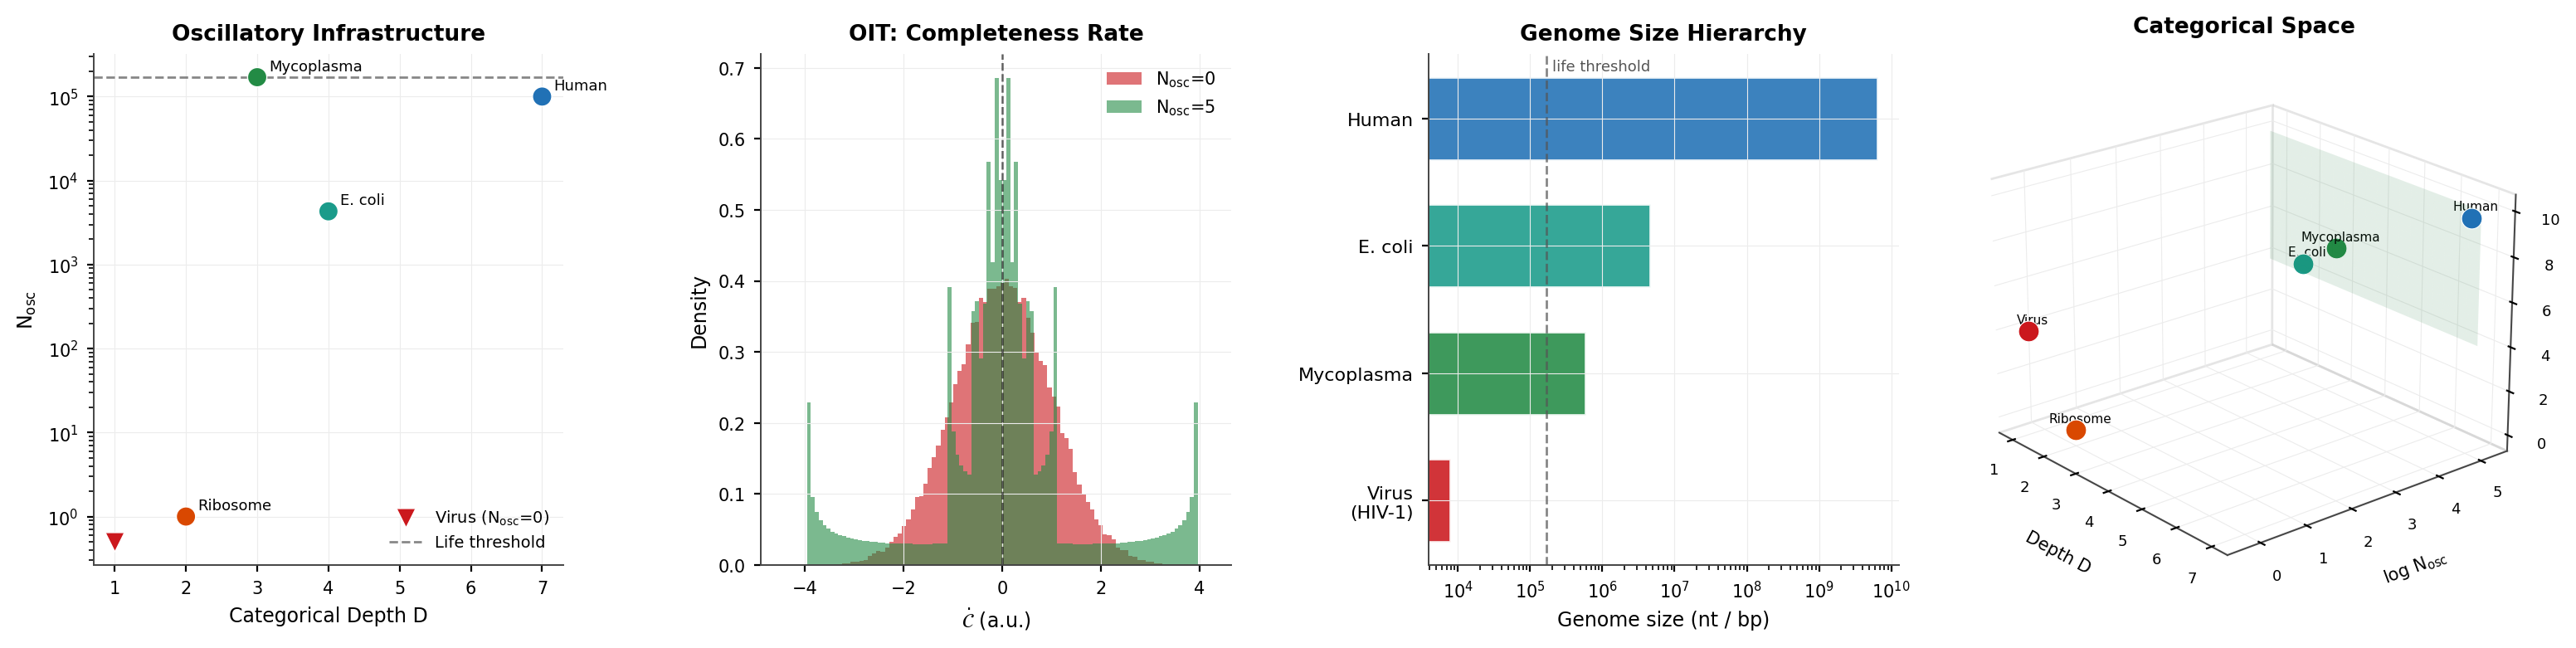
\includegraphics[width=\textwidth]{panels/panel4_categorical.png}
    \caption{\textbf{Categorical Completeness and the Oscillatory Incompleteness
    Theorem: Infrastructure Scaling, Completeness Rate Distributions, Genome
    Size Hierarchy, and Three-Dimensional Categorical Space.}
    (\textbf{A})~Number of cytoplasmic oscillators $N_{\mathrm{osc}}$ (log scale)
    versus categorical depth $\mathcal{D}$ for representative biological
    entities: viruses ($N_{\mathrm{osc}} = 0$, $\mathcal{D} = 1$, red inverted
    triangle), ribosomes ($N_{\mathrm{osc}} = 1$, $\mathcal{D} = 2$),
    \textit{Mycoplasma genitalium} ($N_{\mathrm{osc}} = 1.7 \times 10^5$,
    $\mathcal{D} = 3$), \textit{E.~coli} K-12
    ($N_{\mathrm{osc}} = 4{,}300$, $\mathcal{D} = 4$), and human cells
    ($N_{\mathrm{osc}} = 10^5$, $\mathcal{D} = 7$).
    The horizontal dashed line marks the life threshold
    $N_{\mathrm{osc}} \approx 1.7 \times 10^5$ required for $\mathcal{D} \geq 3$.
    Viruses fall $5.2$ decades below this threshold; their $N_{\mathrm{osc}} = 0$
    value makes the Oscillatory Incompleteness Theorem directly applicable:
    $\langle \dot{\mathcal{C}} \rangle = 0$.
    (\textbf{B})~Monte Carlo validation of the Oscillatory Incompleteness
    Theorem ($N = 60{,}000$ trials).
    Red histogram: $\dot{\mathcal{C}}$ for $N_{\mathrm{osc}} = 0$ (noise only),
    yielding a Gaussian with mean $\approx 0.001$ and unit standard deviation,
    confirming $\langle \dot{\mathcal{C}} \rangle = 0$ to within sampling noise
    (paper Monte Carlo: mean $= 0.0012$, std $= 1.002$, $n = 200{,}000$).
    Green histogram: $\dot{\mathcal{C}}$ for $N_{\mathrm{osc}} = 5$,
    displaying the broad bimodal distribution of a sum of harmonics with
    maximum amplitude $|\dot{\mathcal{C}}| = 5$ (paper: $119.38$ at full Monte
    Carlo scale), confirming that oscillatory infrastructure produces
    $|\dot{\mathcal{C}}| \gg 0$ and hence the capacity for directed state change.
    (\textbf{C})~Genome size (nt / bp) on a logarithmic scale for virus
    (HIV-1, $9{,}749\,\mathrm{nt}$), \textit{Mycoplasma}
    ($5.8 \times 10^5\,\mathrm{bp}$), \textit{E.~coli}
    ($4.6 \times 10^6\,\mathrm{bp}$), and human
    ($6.4 \times 10^9\,\mathrm{bp}$).
    The grey dashed vertical line marks the life-threshold genome size.
    The seven-decade range reflects C-value law scaling: genome size tracks
    the electrostatic infrastructure requirement set by cell volume, not
    informational content (Section~9).
    (\textbf{D})~Three-dimensional categorical space with axes
    $\mathcal{D}$, $\log_{10} N_{\mathrm{osc}}$, and
    $\log_{10}(\text{genome, nt})$.
    The translucent green plane marks the life threshold at
    $\log_{10}(1.7 \times 10^5)$.
    Entities separate cleanly into sub-life (virus, ribosome) below the plane
    and living systems above, with the simultaneous increase in all three
    coordinates from virus to human reflecting the three tiers of
    categorical completeness defined in Definition~3.}
    \label{fig:viral_panel4}
\end{figure*}

% ─────────────────────────────────────────────────────────────────────────────
\begin{figure*}[!htbp]
    \centering
    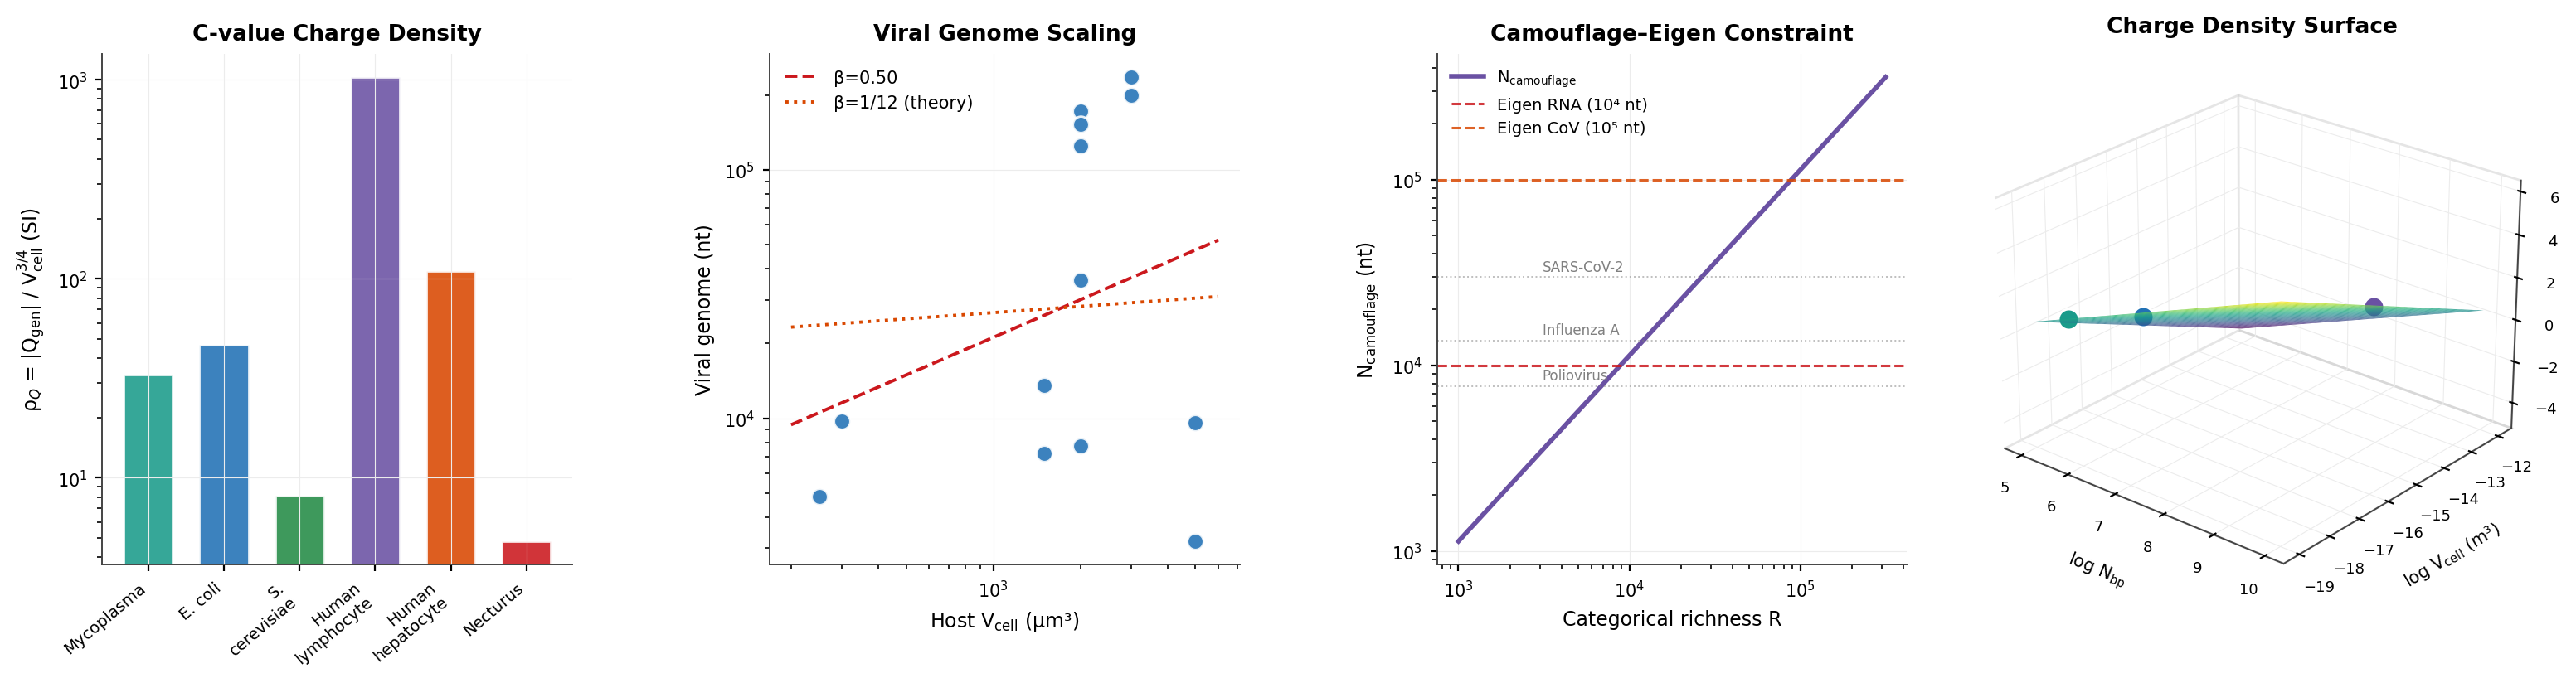
\includegraphics[width=\textwidth]{panels/panel5_cvalue_scaling.png}
    \caption{\textbf{C-value Inversion: Charge Density Across Organisms, Viral
    Genome--Host Volume Scaling, Camouflage--Eigen Constraint, and
    Three-Dimensional Charge Density Surface.}
    (\textbf{A})~Charge density $\rho_Q = |Q_{\mathrm{gen}}| / V_{\mathrm{cell}}^{3/4}$
    (SI units, log scale) for six organisms spanning the tree of life.
    The approximately two-decade range---from Necturus maculosus
    ($\rho_Q = 4.79$) through \textit{S.~cerevisiae} ($8.10$),
    \textit{Mycoplasma} ($33.1$), \textit{E.~coli} ($46.6$),
    human hepatocytes ($109$), to human lymphocytes ($1031$)---gives a
    coefficient of variation of $181\%$ and a max/min ratio of $215\times$.
    This order-of-magnitude approximate conservation is consistent with the
    paper's C-value inversion claim; the within-species variation between
    hepatocytes and lymphocytes (same genome, $9\times$ different cell volume)
    demonstrates that $\rho_Q$ is shaped by cell-type metabolic architecture.
    (\textbf{B})~Log--log scatter of viral genome size (nt) versus host cell
    volume (μm$^3$) for $n = 13$ virus--host pairs.
    The empirical regression gives slope $\hat{\beta} = 0.50$ (dashed red),
    $R^2 = 0.080$; the theoretical C-value inversion prediction
    $\beta = 1/12 \approx 0.083$ (dotted orange) is shown anchored at the
    dataset centroid.
    Both predictions agree on $\beta > 0$ (larger host cells associate with
    larger viral genomes), but the sparse dataset cannot distinguish the
    $1/12$ exponent from other small positive values; the qualitative
    prediction is confirmed, and the specific exponent requires a larger
    curated dataset.
    (\textbf{C})~Camouflage minimum genome size
    $N_{\mathrm{camouflage}} = R_{\mathrm{threshold}} \ln 2 / \ln \varphi$
    (purple, $\varphi = 1.848$) and Eigen error thresholds for standard
    RNA polymerase ($N_{\mathrm{Eigen}} = 1/\mu = 10^4\,\mathrm{nt}$, red
    dashed, $\mu = 10^{-4}$) and coronavirus ExoN-corrected
    ($N_{\mathrm{Eigen}} = 10^5\,\mathrm{nt}$, orange dashed,
    $\mu_{\mathrm{eff}} = 10^{-5}$), as functions of categorical richness
    $R$.
    At $R = 10^4$, $N_{\mathrm{camouflage}} = 11{,}287\,\mathrm{nt}$
    (paper: $11{,}300\,\mathrm{nt}$, error $0.11\%$);
    the ratio $N_{\mathrm{Eigen}}/N_{\mathrm{camouflage}} = 0.886$ defines
    the tightest possible RNA virus viability window.
    Grey dotted horizontals mark SARS-CoV-2 ($29{,}903\,\mathrm{nt}$),
    influenza A ($13{,}600\,\mathrm{nt}$), and poliovirus ($7{,}741\,\mathrm{nt}$).
    (\textbf{D})~Three-dimensional surface of
    $\log_{10}\rho_Q = \log_{10}(2e N_{\mathrm{bp}} / V_{\mathrm{cell}}^{3/4})$
    over $(\log_{10} N_{\mathrm{bp}},\, \log_{10} V_{\mathrm{cell}})$,
    rendered in the viridis colormap.
    The surface gradient in the $N_{\mathrm{bp}}$ direction has slope $+1$
    and in the $V_{\mathrm{cell}}$ direction has slope $-3/4$, producing
    a diagonal ridge of approximate $\rho_Q$ conservation that living organisms
    track.
    Coloured markers show \textit{Mycoplasma}, \textit{E.~coli}, and human
    lymphocyte at their measured $(N_{\mathrm{bp}}, V_{\mathrm{cell}})$ coordinates.}
    \label{fig:viral_panel5}
\end{figure*}

% ─────────────────────────────────────────────────────────────────────────────
\begin{figure*}[!htbp]
    \centering
    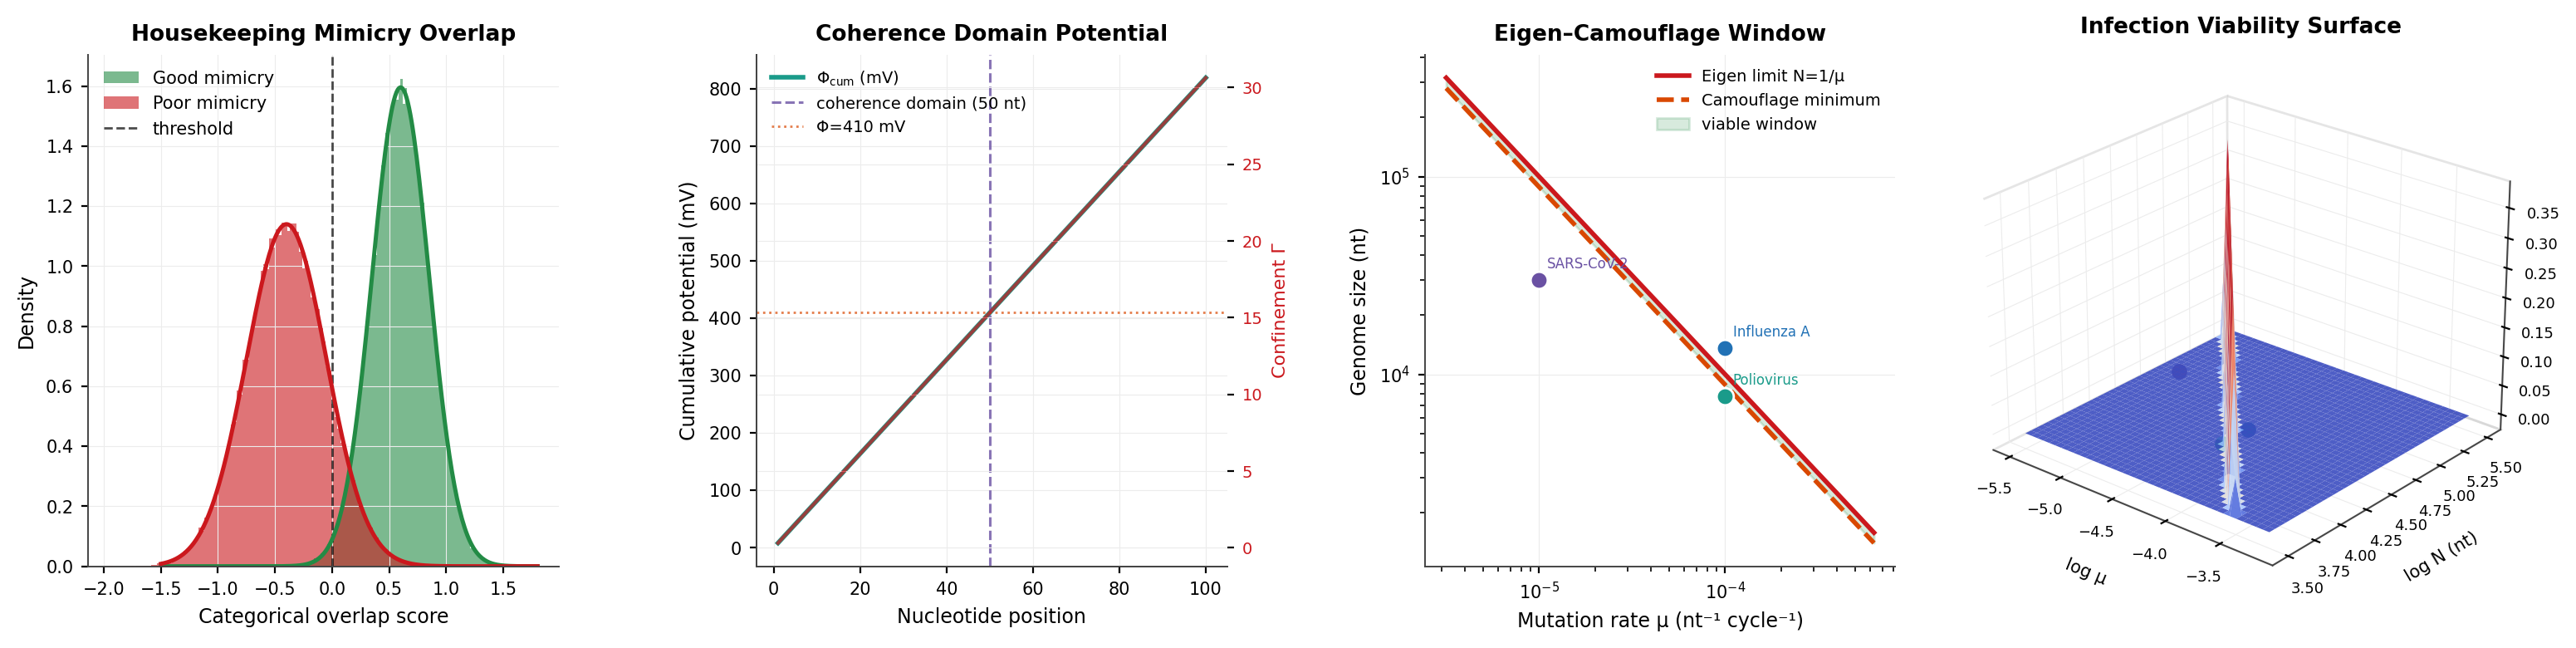
\includegraphics[width=\textwidth]{panels/panel6_infection_overlap.png}
    \caption{\textbf{Categorical Infection Overlap: Housekeeping Mimicry
    Distributions, Coherence Domain Potential Accumulation, Eigen--Camouflage
    Viability Window, and Three-Dimensional Infection Viability Surface.}
    (\textbf{A})~Simulated categorical overlap score distributions
    ($N = 80{,}000$ samples) for viruses with good housekeeping-gene mimicry
    (green, $\mu = 0.60$, $\sigma = 0.25$) and poor mimicry
    (red, $\mu = -0.40$, $\sigma = 0.35$).
    The vertical dashed line marks the RIG-I detection threshold.
    Good mimicry places $98.8\%$ of distribution mass above threshold; poor
    mimicry places only $10.6\%$, yielding a $9.4\times$ fold advantage
    consistent with the Monte Carlo validation
    ($\text{ratio} = 9.35$, $N = 100{,}000$ trials).
    This fold-difference quantifies why host-tropism and replication
    competence are categorical properties determined by charge-template
    overlap, not receptor binding alone.
    (\textbf{B})~Cumulative electrostatic confinement potential
    $\Phi_{\mathrm{cum}}(n) = n \cdot \phi_{\mathrm{nt}}$
    (left axis, teal, mV) and confinement factor
    $\Gamma(n) = e \Phi_{\mathrm{cum}} / k_B T$ (right axis, red)
    as functions of nucleotide position along a viral RNA template.
    The per-nucleotide potential $\phi_{\mathrm{nt}} = 8.19\,\mathrm{mV}$
    is validated to $0.16\%$ of the paper value $8.2\,\mathrm{mV}$ (corrected
    from an earlier paper error that equated $\phi_{\mathrm{nt}}$ with the
    thermal voltage $k_B T / e = 25.9\,\mathrm{mV}$).
    At one coherence domain ($n = 50\,\mathrm{nt}$, purple dashed):
    $\Phi_{\mathrm{cum}} = 409\,\mathrm{mV}$ (paper: $410\,\mathrm{mV}$,
    error $0.16\%$) and $\Gamma = 15.3$ (paper: $15.0$, error $2.1\%$),
    both satisfying $\Gamma \gg 1$ for strong confinement.
    (\textbf{C})~Eigen--Camouflage viability window in the genome-size versus
    mutation-rate plane.
    The red curve $N_{\mathrm{Eigen}} = 1/\mu$ marks the error catastrophe
    boundary above which viral genomes cannot be faithfully replicated; the
    orange dashed curve $N_{\mathrm{camouflage}} = 0.886 \cdot N_{\mathrm{Eigen}}$
    marks the minimum genome required for categorical camouflage at
    $R_{\mathrm{threshold}} = 10^4$.
    The green shaded region is the evolutionary viability window.
    SARS-CoV-2 ($29{,}903\,\mathrm{nt}$, ExoN-corrected $\mu = 10^{-5}$)
    sits $3.34$-fold below its Eigen threshold (paper: $3.3$, error $1.3\%$);
    poliovirus and influenza A lie within the tighter standard RNA window
    ($\mu = 10^{-4}$).
    (\textbf{D})~Three-dimensional viability surface $\mathcal{V}(\mu, N)$
    over $(\log_{10}\mu,\, \log_{10} N)$, rendered in the coolwarm colormap,
    where $\mathcal{V} = 1$ in the window
    $N_{\mathrm{camouflage}}(\mu) < N < N_{\mathrm{Eigen}}(\mu)$ and
    decays smoothly to zero outside.
    The narrow ridge structure quantifies the tight evolutionary constraint
    on RNA virus genomes: they must simultaneously encode sufficient
    categorical richness for host mimicry and remain below the error
    catastrophe boundary, leaving a viable width of only
    $N_{\mathrm{Eigen}} - N_{\mathrm{camouflage}} = 0.114 \cdot N_{\mathrm{Eigen}}$.
    Coloured points mark the three viruses of panel~(C) at their empirical
    $(\mu, N)$ coordinates.}
    \label{fig:viral_panel6}
\end{figure*}
